\chapter{Graph Theory}

\section{Basic concepts}

\subsection{Graph}

\begin{itemize}
\item A graph $G = (N, E)$ with $N$ a set of nodes and $E$ a set of edges, swhere an edge is a pair of two nodes.
\item Example : $N = {a, b, c}, E = {{a, b}, {b, c}}$
\end{itemize}

\subsection{Directed Graph}

\begin{itemize}
\item Each edge has a direction, and is represented as a tuple with a \textit{first} and a \textit{second}
\item Example : $E = {(a, b), (b, c)}$
\end{itemize}

\subsection{Undirected Graph}

\begin{itemize}
\item Edges have no direction, they are represented as a set
\item Example : $E = {{a, b}, {b, c}}$
\end{itemize}

\section{Paths and connectivity}

\subsection{Path}

A path in a graph is a sequence of nodes such that each successive pair in the sequence is an edge of the graph.

\subsection{Simple path}

A simple path is a path where each node occurs at most once.

\subsection{Cycle}

A cycle is a path with 3 or more edges such that the first and last nodes are the same and otherwise all node are distinct.

\subsection{Connected Graph}

A graph is connected if there exists a path between every pair of nodes.

\subsection{Component of a graph}

A component is a subset of nodes that satisfies two properties :
\begin{enumerate}
\item The subset is \textit{connected}.
\item The subset is \textit{maximal} : there is no superset that is connected.
\end{enumerate}

\subsubsection{Strongly connected component}

A component is strongly connected if it satisfies two properties :
\begin{enumerate}
\item Each node in the subset has a path to each other node in the subset.
\item The subset is \textit{maximal} : it is not part of a larger subset with the property that each node can reach the other.
\end{enumerate}

\subsection{Analyzing a graph}

\begin{itemize}
\item A graph can be divided into its components.
\item For each component, we can study its internal structure. For example, removing a node (with its edges) may split it in more components.
\end{itemize}

\subsection{Giant components}

Large social networks often have a giant component, which is a component that contains a significant fraction of the graph's nodes.

\subsection{Bipartite graph}

A bipartite graph is a graph where the nodes can be separated into two sets such that each edge connects a node from one set to the other.

\subsection{Clique or complete graph}

There exist an edge joining every pair of nodes.

\subsubsection{Labeled complete graph}

A complete graph where every edge is labeled.

\section{Distance in a graph}

\subsection{Length}

The length of a path is the number of edges it contains.

\subsection{Distance between two nodes}

Length of the shortest path between these two nodes.

\subsection{Breadth-first-search}

For finding distances between nodes.

\chapter{How to combine graph theory and sociology}

\section{Social networks}

A graph where the nodes denote human beings and the edges denote a connection between two human beings.

\subsubsection{Triadic closures}

\begin{figure}[H]
    \centering
    \includegraphics[width=0.4\textwidth]{triadic_closure}
\end{figure}

if two people in a social network have a common friend, then the likelihood that they will become friends in the future is increased :

\begin{itemize}
\item B and C have more opportunities to meet.
\item B and C both thrust A so they have a basis for trusting each other.
\item B and C have common interests with A so they may have common interests with each other.
\item A has an incentive to bring B and C together since if they are not friends, it stresses A.
\end{itemize}

\subsubsection{Strong triadic closure}

If A and B are close friends as well as A and C, then it is especially likely that B and C will become connected.

\subsection{Clustering coefficient}

\begin{figure}[H]
    \centering
    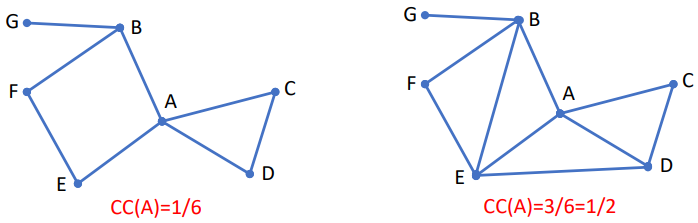
\includegraphics[width=0.5\textwidth]{clust_coef}
\end{figure}

The \textit{clustering coefficient} $CC(A)$ of node A in a graph is :
\begin{itemize}
\item $CC(A) =$ probability that two randomly selected friends of A are friends with each other.
\item $CC(A) = \frac{X}{Y}$
	\begin{itemize}
	\item $X =$ the number of pairs of A's friends that are connected.
	\item $Y =$ the maximum number of pairs of A's friends that are connected.
	\end{itemize}
\item Triadic closures causes the clustering coefficient to increase
\end{itemize}

\subsection{Bridges}

\begin{figure}[H]
    \centering
    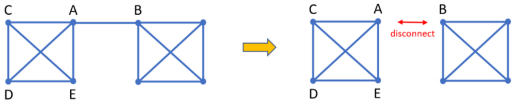
\includegraphics[width=0.5\textwidth]{bridge}
\end{figure}

The edge joining A and B is a \textit{bridge} if removing this edge causes A and B to be in different components.

\subsubsection{Local bridges}

\begin{figure}[H]
    \centering
    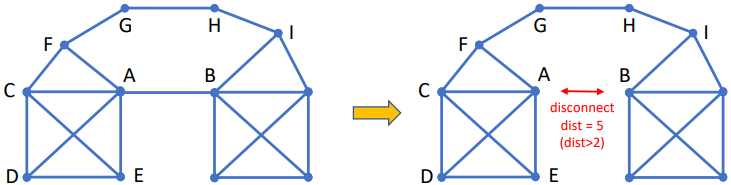
\includegraphics[width=0.5\textwidth]{local_bridge}
\end{figure}

\begin{itemize}
\item The edge joining A and B is a \textit{local bridge} if A and B have no friends in common, so deleting the edge will increase the distance between A and B to a value \textit{strictly greater than 2}.
\item Local bridges play roughly the same role as bridges, but in a less extreme way : they connect a node to another node that would otherwise be far away.
\end{itemize}

\subsection{Neighborhood overlap}

The neighborhood overlap generalizes local bridges :
$\frac{X}{Y}$ where
\begin{itemize}
\item $X =$ number of nodes who are neighbors of \textit{both} A and B.
\item $Y =$ number of nodes who are neighbors of \textit{at least one} of A and B.
\end{itemize}

\chapter{Networks in their surrounding context}

\section{Longitudinal studies}

The network must be followed over time.

\section{Homophily}

They are two basic mechanisms that cause friends to resemble each other : selection and social influence (both are sociological concepts)
\begin{itemize}
\item \textit{Selection} : people select friends with similar characteristics (an internal mechanism).
	\begin{itemize}
	\item individuals drive the formation of new links.
	\end{itemize}
\item \textit{Social influence} : people modify their behaviors to be closer to their friends (an external mechanism), also called "peer pressure".
	\begin{itemize}
	\item Existing links drive the formation of new links
	\end{itemize}
\end{itemize}

\subsection{Affiliation network}

\begin{figure}[H]
    \centering
    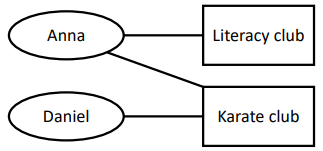
\includegraphics[width=0.35\textwidth]{affiliation_network}
\end{figure}

An affiliation network is a bipartite graph that shows which individuals are affiliated with which activities.
\begin{itemize}
\item The first set is the individuals.
\item The second set is the foci.
\end{itemize}

\subsubsection{Three forms of closures in a social-affiliation network}

\begin{figure}[H]
    \centering
    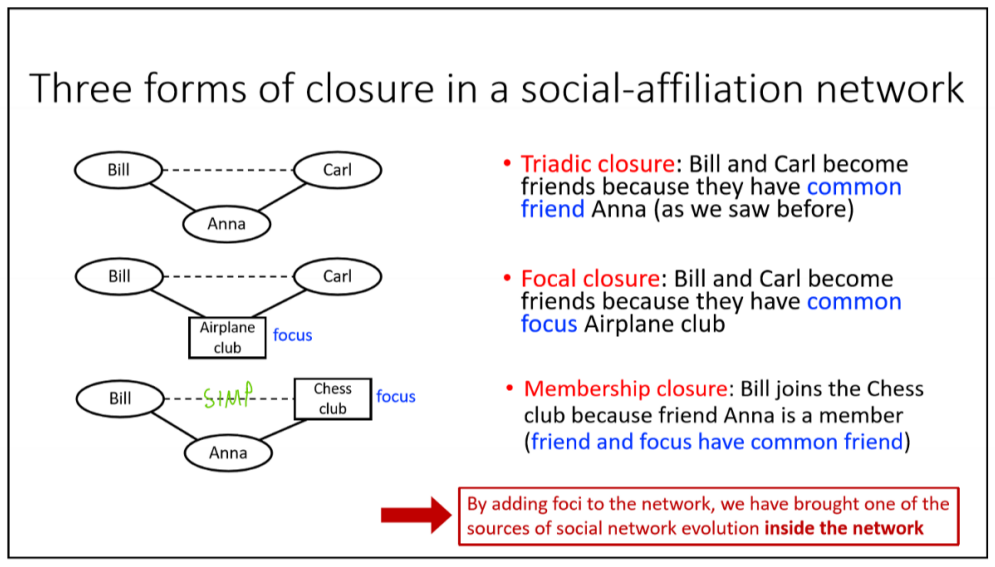
\includegraphics[width=0.7\textwidth]{closures_types}
\end{figure}

\subsection{Measuring homophily}

\begin{figure}[H]
    \centering
    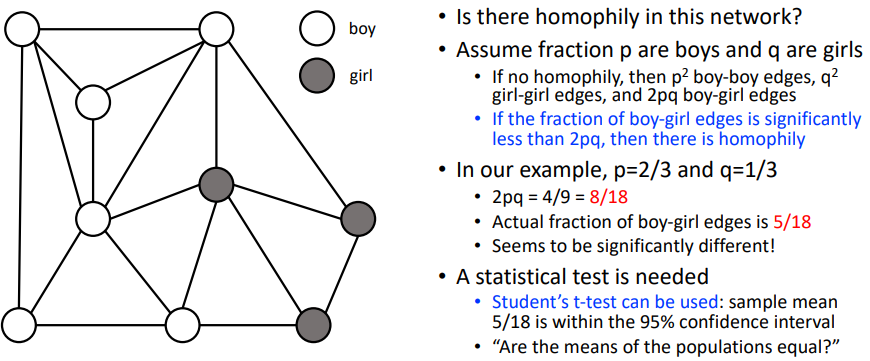
\includegraphics[width=0.8\textwidth]{homophilie_calc}
\end{figure}

\chapter{Positive and negative relationships}

\section{Structural balance}

\subsection{Balanced and unbalanced triangles}

\begin{figure}[H]
    \centering
    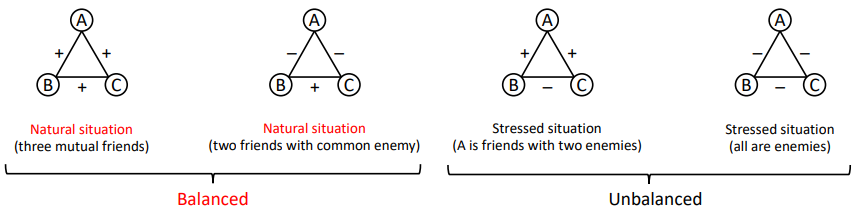
\includegraphics[width=0.6\textwidth]{balanced_unbalanced}
\end{figure}

\subsection{Balance for networks}

\subsubsection{Local definition}

A network is balanced if all the triangles in it are balanced

\subsubsection{Global definition}

If a labeled complete graph is balanced, then either all pairs of nodes are friends, or else the nodes can be divided into two groups such that nodes within a group are friends and nodes between groups are enemies.

\subsection{Weak structural balance}

\subsubsection{Local definition}

A network is balanced if all the triangles in it are balanced or they are (---).

\subsubsection{Global definition}

If a labeled complete graph is weakly balanced, then its nodes can be divided into groups such that any two nodes belonging to the same group are friends and any two nodes belonging to different groups are enemies.

\subsubsection{Degrees of structural balance}

\begin{figure}[H]
    \centering
    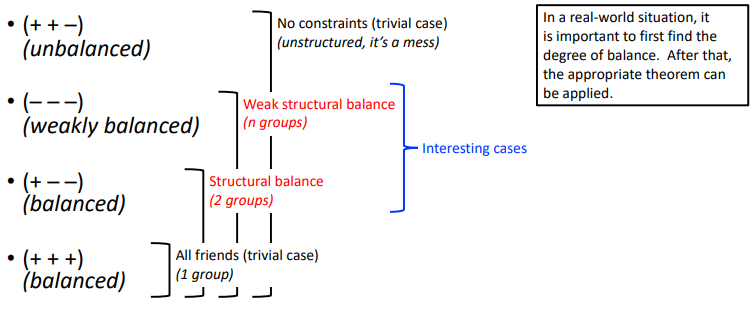
\includegraphics[width=0.6\textwidth]{degree_structural_balance}
\end{figure}

\chapter{Introduction to game theory}

Game theory studies the interaction of participants.

\section{Game with two rational player}

\subsection{Game}

\begin{itemize}
\item There is a set of participants, called the players.
\item Each player has a set of options for how to behave : we will refer to these options as the player's strategies.
\item For each choice of strategies (one by each player), each player receives a payoff. The payoff depends on the strategies selected by all players. Payoffs are generally numbers, and each player prefers larger payoffs to smaller ones.
\end{itemize}

\subsubsection{Assumptions}

\begin{enumerate}
\item All that a player care about is summarized in the payoff.
\item Each player knows everything about the game.
\item Each player chooses a strategy to maximize their own payoff, given a belied about the strategy ysed be the other player.
\end{enumerate}

\subsubsection{On shot game}

Two players that play only once and where the players simultaneously and independently choose their actions.

\subsubsection{Dynamic games}

Games that are played sequentially over time.

\subsubsection{Forms}

\paragraph{Normal form}

In normal form, each player commits ahead of time to a complete plan for playing the whole game.

\begin{figure}[H]
    \centering
    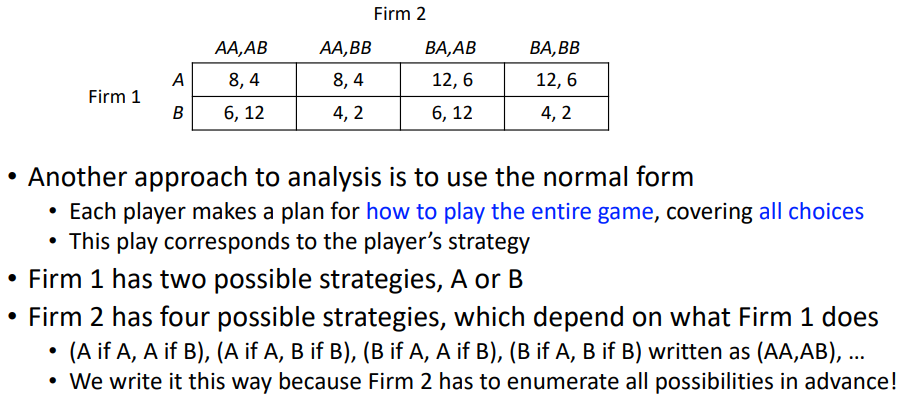
\includegraphics[width=0.6\textwidth]{normal_form}
\end{figure}

\paragraph{Extensive form}

In extensive form, each player makes an optimal decision at each intermediate step.

\begin{figure}[H]
    \centering
    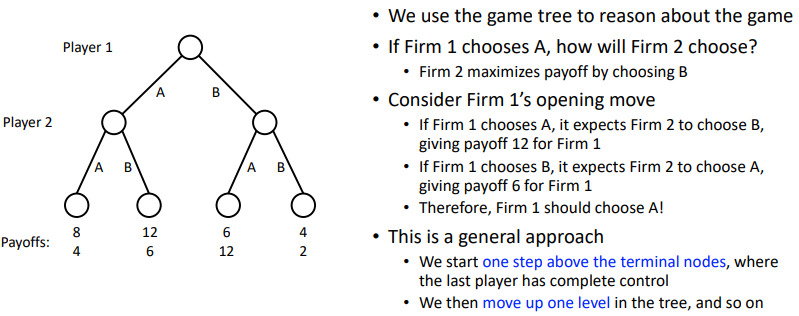
\includegraphics[width=0.7\textwidth]{extensive_form}
\end{figure}

\subsection{Strategies}

\subsubsection{Strictly dominant strategy}

When a player has a strategy strictly better than all others, regardless of what the other player does (not always possible).

\begin{table}[H]
    \centering
    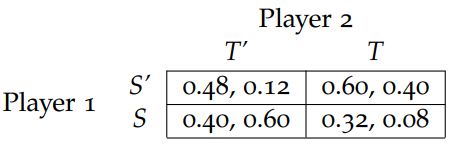
\includegraphics[width=0.35\textwidth]{strictly_dominant_strategy}
\end{table}

\subsubsection{Mixed strategies}

We introduce randomness.

\begin{table}[H]
    \centering
    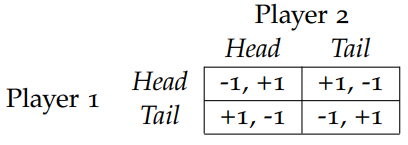
\includegraphics[width=0.35\textwidth]{mixed_strategies}
\end{table}

\subsubsection{Best response}

\begin{table}[H]
    \centering
    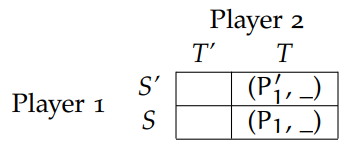
\includegraphics[width=0.25\textwidth]{best_response}
\end{table}

\begin{itemize}
\item S for player 1 is best response to T for Player 2 if :
	\begin{itemize}
	\item For all other strategies, $S'$ of Player 1 : $P1(S, T) \geq P1(S', T)$
	\end{itemize}
\item S for player 1 is strictly best response to T for Player 2 if :
	\begin{itemize}
	\item For all other strategies, $S'$ of Player 1 : $P1(S, T) > P1(S', T)$
	\end{itemize}
\end{itemize}

\subsubsection{Nash equilibrium}

\begin{itemize}
\item Each player's strategy is a best response to the other.
\item Corresponds to free market.
\end{itemize}

\begin{table}[H]
    \centering
    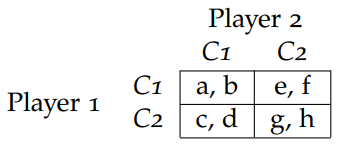
\includegraphics[width=0.28\textwidth]{nash_equilibrium}\\
    $P(C2, C1)$ is a Nash equilibrium if $a < c$ and $h < d$
\end{table}

\paragraph{Coordination / anti-coordination games}

Games with multiple Nash equilibria.

\subsubsection{Pareto optimality}

\begin{itemize}
\item A choice of strategies (one by each player) is Pareto optimal if there is no other choice in which all players receive payoffs at least as high, and at least one player receives a strictly higher payoff.
\item Corresponds to regulation.
\end{itemize}

\begin{table}[H]
    \centering
    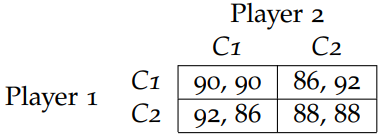
\includegraphics[width=0.3\textwidth]{nash_pareto}\\
    $(88, 88)$ is a Nash equilibrium, whereas the 3 others options are Pareto optimal.
\end{table}

\subsubsection{Social optimality}

\begin{itemize}
\item A choice of strategies (one by each player) is \textcolor{orange}{socially optimal} if it maximizes the sum of the players' payoff.
\item It is also Pareto optimal.
\end{itemize}

\section{Summary}

\begin{figure}[H]
    \centering
    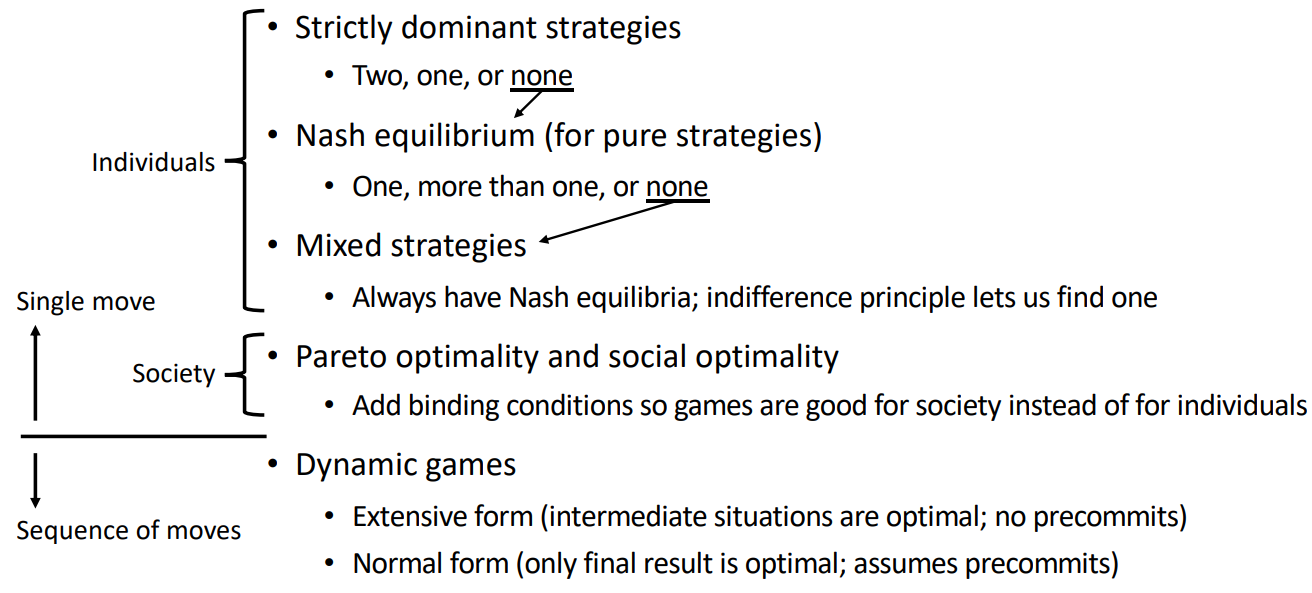
\includegraphics[width=0.8\textwidth]{game_theory_sum}
\end{figure}

\chapter{Car traffic networks}

\section{Braess' Paradox}

\begin{figure}[H]
    \centering
    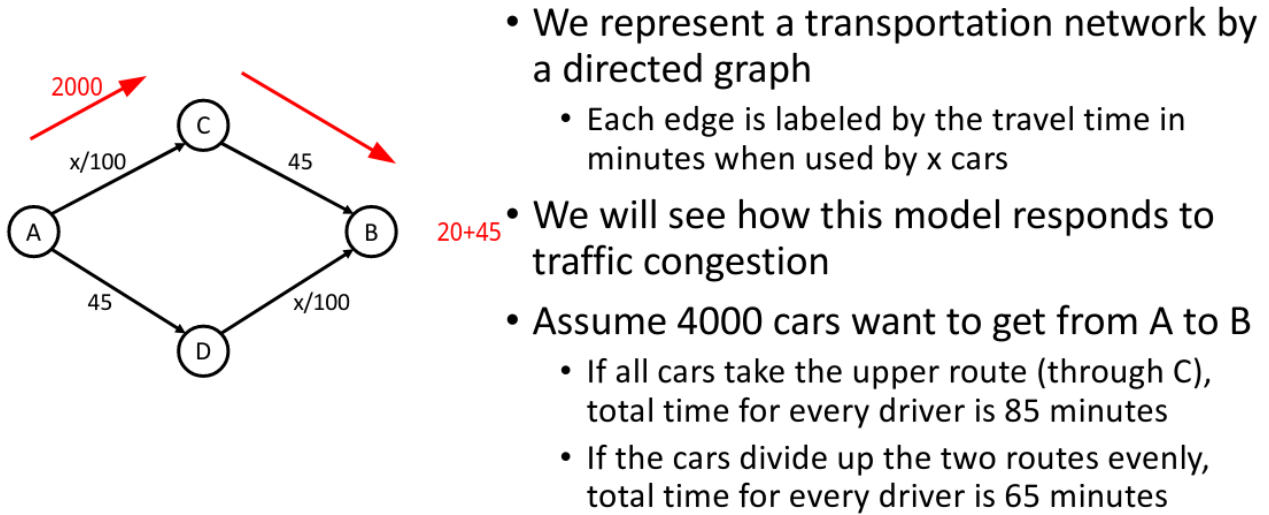
\includegraphics[width=0.8\textwidth]{braess_1}
\end{figure}

\begin{figure}[H]
    \centering
    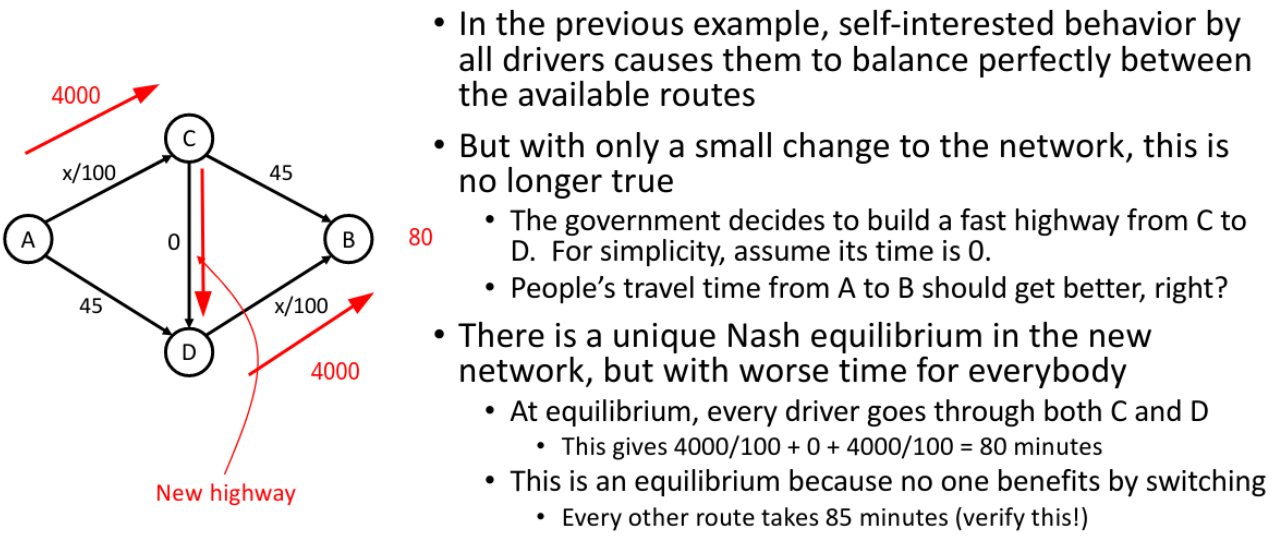
\includegraphics[width=0.82\textwidth]{braess_2}
\end{figure}

There is no paradox because there are many situations where adding more choices leads to worse situations.

\chapter{Auctions}

\section{When are auctions appropriate ?}

When the value of the objet is :
\begin{itemize}
\item \textcolor{orange}{known} : an auction is \textcolor{orange}{inappropriate}.
\item \textcolor{orange}{unknown} : an auction is \textcolor{orange}{appropriate}.
\end{itemize}

\subsection{Two kind of unknown values}

\subsubsection{Independent, private value}

\begin{itemize}
\item Each buyer is interested for its own personal use
\item The values can be different because the buyers have different tastes
\end{itemize}

\subsubsection{Common value}

\begin{itemize}
\item Assume each buyer plans to resell the item if bought, then the item has an unknown but common value regardless of who buys it.
\item \textcolor{orange}{Winner's course} : if there are many bidders, the winning bidder will very likely overestimate the common value and lose money on the resell of the object.
	\begin{itemize}
	\item[$\rightarrow$] To counter it, we should bid lower that our private value of the good.
	\end{itemize}
\end{itemize}

\section{Type of auctions}

\subsection{Ascending-bid auctions}

\begin{itemize}
\item English auctions.
\item Realtime.
\item Seller gradually raises the price until only one bidder remains.
\item Equivalent to second-price auctions.
\end{itemize}

\subsection{Descending-bid auctions}

\begin{itemize}
\item Dutch auctions.
\item Realtime.
\item Seller gradually lowers the price until the first bidder accepts.
\item Equivalent to first-price auctions.
\end{itemize}

\subsection{First-price sealed-bid auctions}

\begin{itemize}
\item Simultaneous bids.
\item The highest bidder wins and pays the value of their id.
\item Payoff to bidder $i$ with value $v_i$ and bid $b_i$ is defined as follows :
	\begin{itemize}
	\item if $b_i$ is not the winning bid, then the payoff to $i$ is $0$.
	\item if $b_i$ is the winning bid, then the payoff to $i$ is $(v_i - b_i)$.
	\end{itemize}
\end{itemize}

\subsection{Second-price sealed-bid auctions}

\begin{itemize}
\item Vickrey auctions.
\item Simultaneous bids.
\item The highest bidder wins and pays the vale of the second-highest bid.
\item Bidding your \textcolor{orange}{true value} is a \textcolor{orange}{dominant strategy}.
\item Payoff to bidder $i$ with value $v_i$ and bid $b_i$ is defined as follows :
	\begin{itemize}
	\item if $b_i$ is not the winning bid, then the payoff to $i$ is $0$.
	\item if $b_i$ is the winning bid, and some other $b_j$ is the second-place bid, then the payoff to $i$ is $(v_i - b_j)$.
	\end{itemize}
\end{itemize}

\begin{figure}[H]
    \centering
    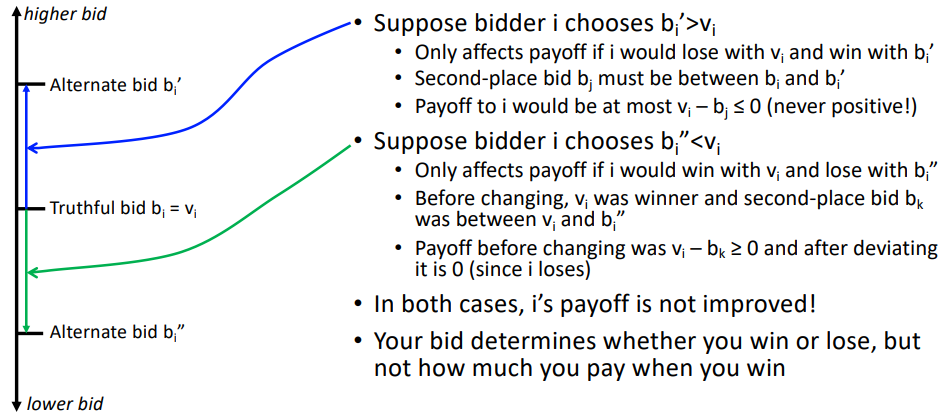
\includegraphics[width=0.82\textwidth]{second_price_proof}
\end{figure}

\chapter{Markets}

A market is :
\begin{itemize}
\item any place where two or more parties can meet to exchange goods or services, usually for money but sometimes directly through barter.
\item a coordinating mechanism that uses prices to convey information among the parties to regulate production and distribution.
\end{itemize}

\section{Matching markets}

A matching market is a market that matches each buyer to a desired item.

\subsection{Perfect matching}

If there are an equal number of nodes on each side of a bipartite graph, then a perfect matching is an assignment between sides such that :
\begin{enumerate}
\item Each node is connected by an edge.
\item No two left nodes are assigned to the same right nodes.
\end{enumerate}

\begin{figure}[H]
    \centering
    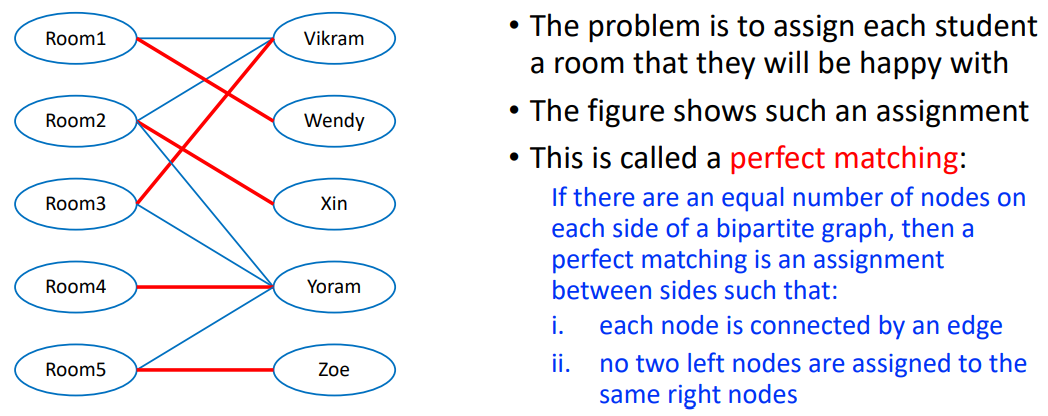
\includegraphics[width=0.6\textwidth]{perfect_matching}
\end{figure}

\subsection{Constricted sets}

Given any set $S$ of nodes on the right side, we define the neighbor set $N(S)$ as the collection of all corresponding left nodes. Set $S$ is constricted if $|N(S)| < |S|$.

\begin{figure}[H]
    \centering
    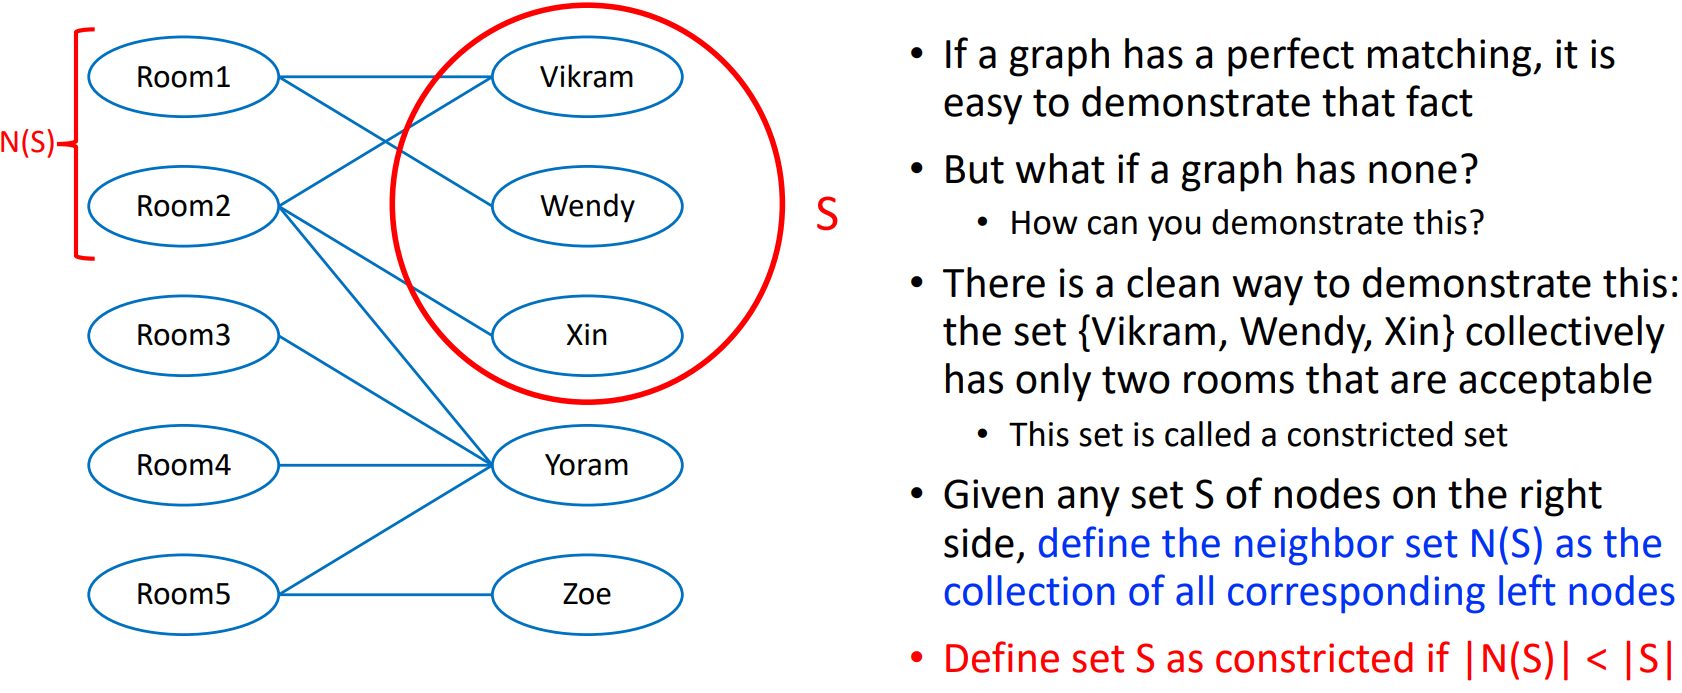
\includegraphics[width=0.6\textwidth]{constricted_set}
\end{figure}

\subsection{Matching theorem}

\begin{formal}
If a bipartite graph with equal numbers of left and right nodes has no perfect matching, then it must contain a constricted set.
\end{formal}

\subsection{Matching markets with prices}

\subsubsection{Prices and market clearing}

\paragraph{Market clearing}

\begin{itemize}
\item \textcolor{orange}{Market clearing} means that the \textcolor{orange}{supply of an item is equal to the demand}, so that there is no leftover of either.
\item We say that \textcolor{orange}{a set of prices is market clearing if the resulting preferred-seller graph has a perfect matching}.
\item In a bipartite matching market, there exists a set of market-clearing prices for any set of buyer valuations.
\item \textcolor{orange}{Market-clearing prices are always socially optimal} :
	\begin{itemize}
	\item For any st of market-clearing prices in a bipartite matching market, a perfect matching in the preferred-seller graph has the maximum total payoff for sellers and buyers, for any assignment of sellers to buyers.
	\end{itemize}
\end{itemize}

\paragraph{Constructing market clearing prices}

We construct a procedure that gradually increase prices and we show that this will always lead to market clearing.

\begin{figure}[H]
    \centering
    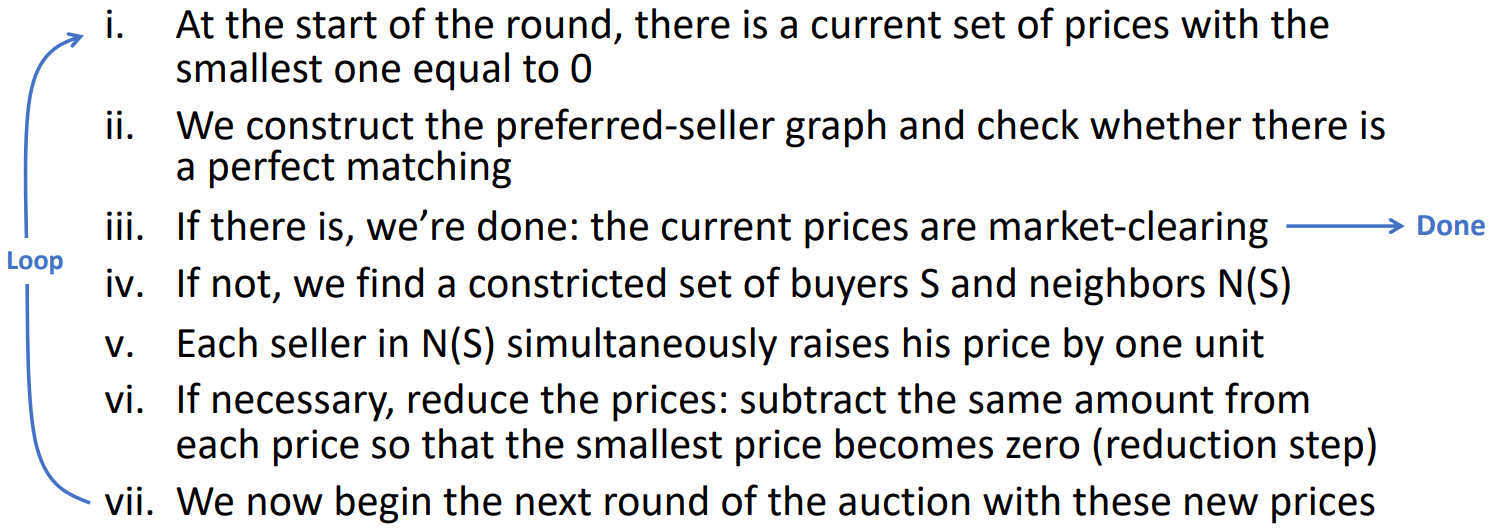
\includegraphics[width=0.8\textwidth]{market_clearing_round}
\end{figure}

\subsection{Auctions and markets are related}

The bipartite matching market generalize an ascending-bid auction :
\begin{itemize}
\item The ascending-bid auction has $n$ buyers and $1$ seller. The seller keeps increasing prices until one buyer wins the auction.
\item The bipartite matching market has $n$ and $n$ sellers. The sellers keep increasing the prices until each buyer has found one seller.
\end{itemize}

\subsubsection{Valuations}

Each person gives a numerical value to each item.

\subsubsection{Quality}

The sum of all persons' valuations.

\subsubsection{Optimal assignment}

It is an assignment of highest possible quality.

\subsection{Summary}

\begin{figure}[H]
    \centering
    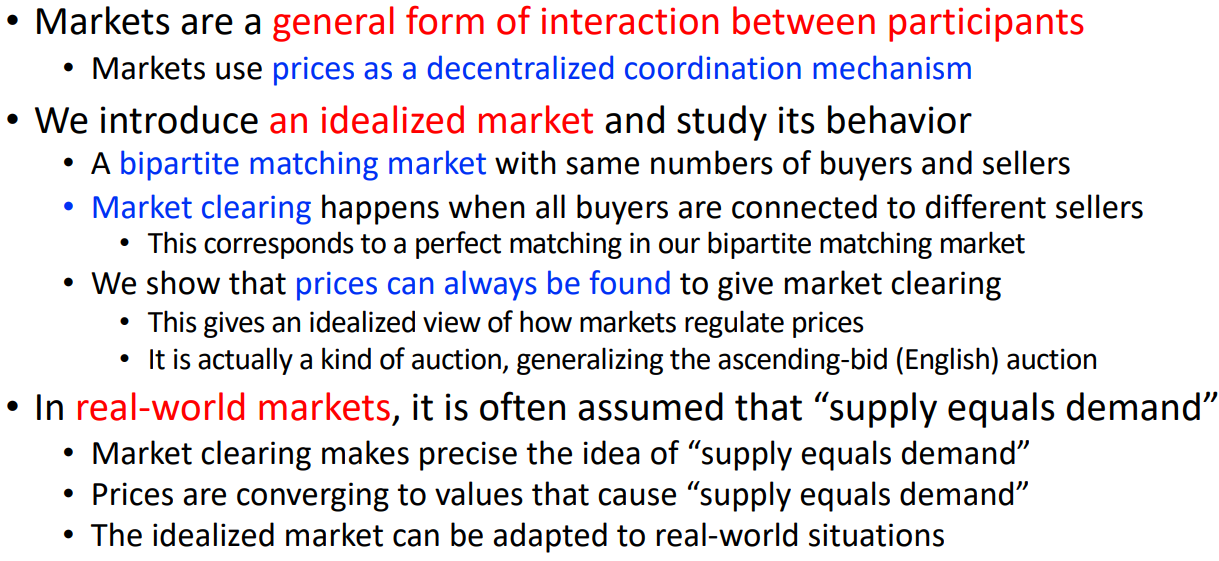
\includegraphics[width=0.8\textwidth]{matching_market_sum}
\end{figure}

\section{Markets with intermediaries}

\subsection{Order book}

Is a list of orders that buyers and sellers hae submitted.

\begin{itemize}
\item \textcolor{orange}{Ask} : lowest sell offer.
\item \textcolor{orange}{Bid} : highest buy offer.
\end{itemize}

\subsection{Buyers, Sellers and Traders}

\subsubsection{Three fundamental principles}

\begin{enumerate}
\item Individual buyers and sellers trade through intermediaries.
\item Buyers and sellers may have access to different intermediaries.
\item Buyers and sellers may trade a different prices.
\end{enumerate}

\subsubsection{Prices depend on the positions in the network}

If a buyer can :
\begin{itemize}
\item only access one trader, then the trader increases his payoff.
\item access several traders, then the buyer increases his payoff.
\end{itemize}

\subsubsection{Prices and the flow of goods}

\begin{enumerate}
\item First step :
	\begin{itemize}
	\item Each trader $t$ offers a bid price $b_{ti}$ to each seller $i$ he his connected to.
		\begin{itemize}
		\item[$\rightarrow$] This is where the strategic reasoning is done.
		\end{itemize}
	\item Each trader $t$ offers an ask price $a_{tj}$ to each buyer $j$ he is connected to.
	\end{itemize}
\item Second step :
	\begin{itemize}
	\item Each seller and buyer chooses at most one trader to deal with.
		\begin{itemize}
		\item[$\rightarrow$] The one with the best offer.
		\end{itemize}
	\item Each seller sells a copy (or not).
	\item Each buyer buys a copy (or not).
	\end{itemize}
\end{enumerate}

\textcolor{orange}{At most} one copy of the good moves along any edge in the network.

\begin{itemize}
\item Many goods can pass through one trader.
\item A trader sells exactly what he receives.
\end{itemize}

\begin{figure}[H]
    \centering
    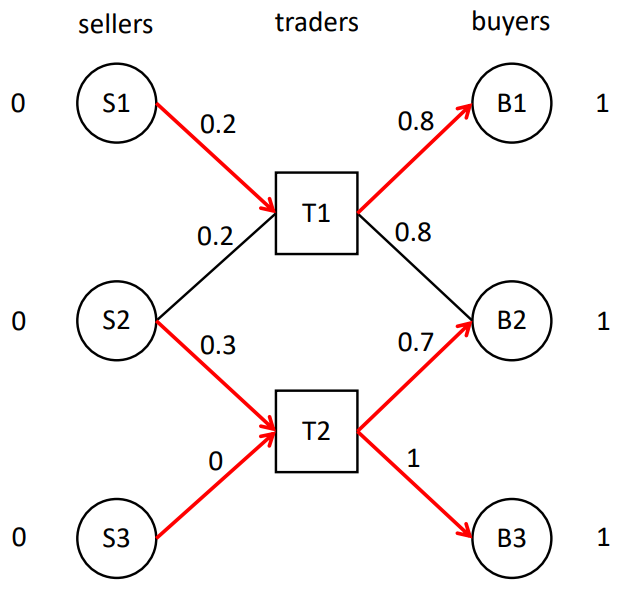
\includegraphics[width=0.4\textwidth]{flow_of_goods}
\end{figure}

Sometimes prices are \textcolor{orange}{pushed to the limit} so there is \textcolor{orange}{no payoff}.

\subsubsection{Indifference}

\begin{itemize}
\item Prices are pushed to the limit of an individual's willingness to trade.
\item We allow trades with zero payoff with ties broken as needed.
\end{itemize}

\subsubsection{Strategies}

\begin{itemize}
\item All traders simultaneously choose ask and bid prices.
\item A seller or buyer's strategy is a choice of neighboring trader (or not).
\end{itemize}

\subsubsection{Payoff}

\begin{itemize}
\item A \textcolor{orange}{trader's payoff} is his total profit : sum of all ask prices of accepted offers to buyers minus sum f bid prices of accepted offers to seller.
\item For \textcolor{orange}{seller} $i$, payoff from selecting trader $t$ is $b_{ti}$, while payoff from selecting no trader is $0$ (note we only consider when $v_i = 0$).
\item For \textcolor{orange}{buyer} $j$, payoff from selecting trader $t$ is $v_j - a_{tj}$ while payoff from selecting no trader is $0$. in the former case, buyer receives the goods but pays $a_{yj}$.
\end{itemize}

\begin{figure}[H]
    \centering
    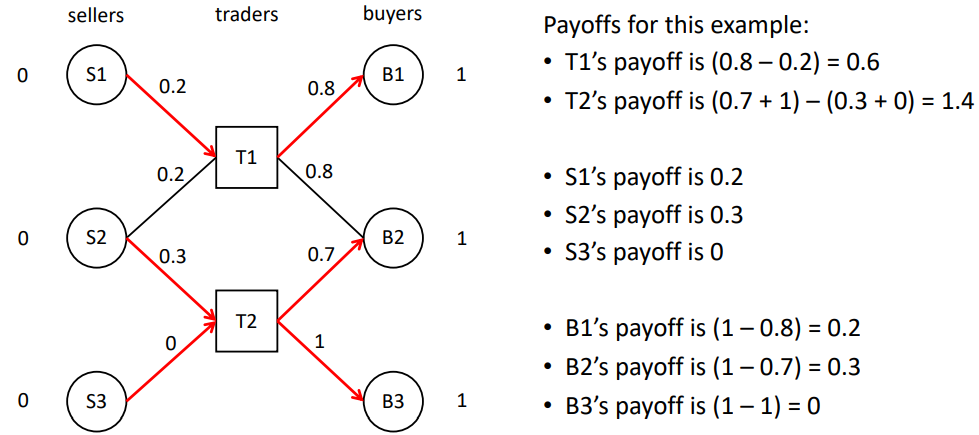
\includegraphics[width=0.7\textwidth]{flow_of_goods_payoff}
\end{figure}

\subsection{Equilibria in trading networks}

\begin{figure}[H]
    \centering
    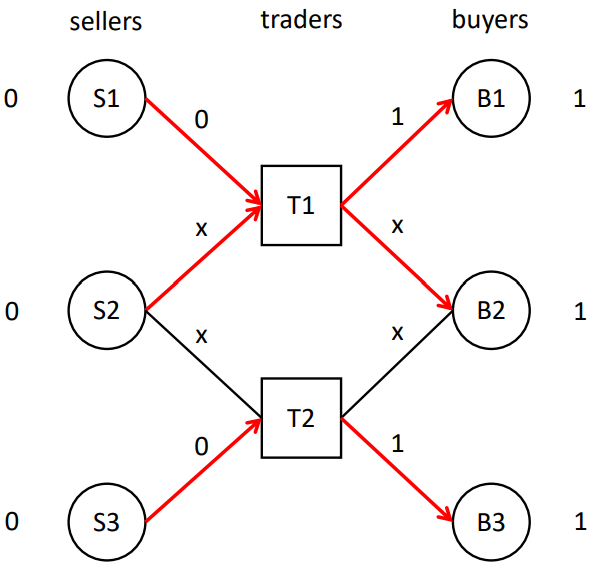
\includegraphics[width=0.4\textwidth]{equilibria_networks}
\end{figure}

\subsubsection{Monopoly}

\begin{itemize}
\item Buyers and sellers are subject to \textcolor{orange}{monopoly} when they access \textcolor{orange}{only a single trader}.
\item The \textcolor{orange}{only equilibrium} is for the trader to \textcolor{orange}{set bid to $0$ to the seller and ask $1$ to the buyer}.
\end{itemize}

\subsubsection{Perfect competition}

\begin{itemize}
\item Buyers and sellers are subject to \textcolor{orange}{perfect competition when they access more than one trader}.
\item Equilibrium for $T2$ occurs at \textcolor{orange}{common bid and ask of x}.
\end{itemize}

\subsubsection{Second-price auction}

\begin{figure}[H]
    \centering
    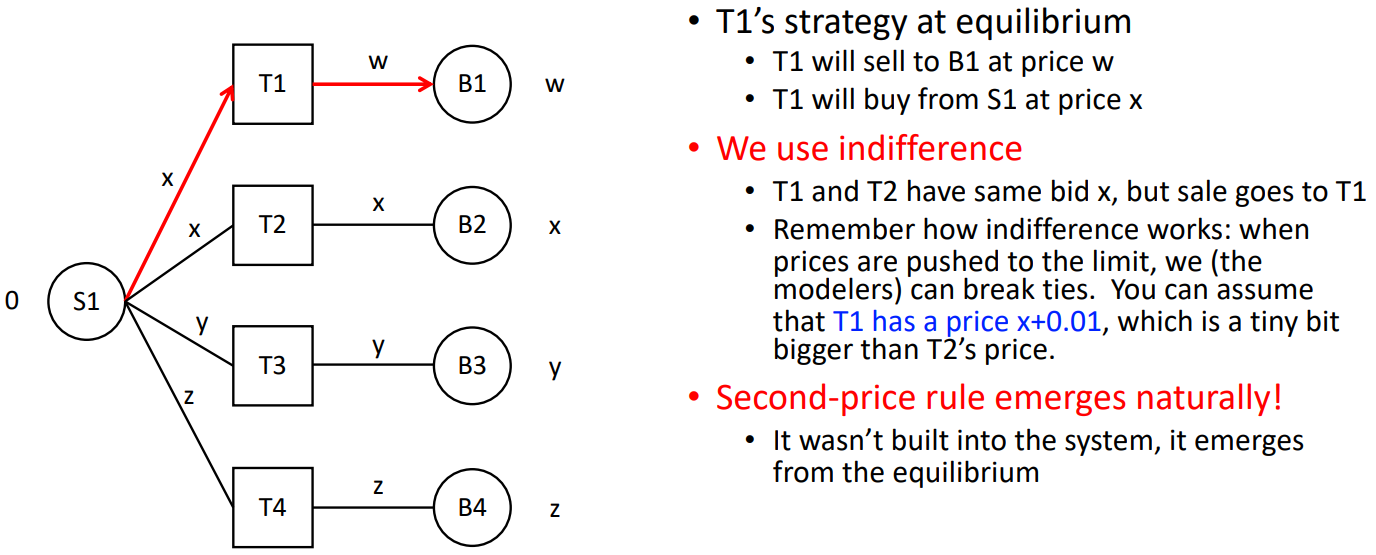
\includegraphics[width=0.7\textwidth]{second_price_auction}
\end{figure}

\subsubsection{Ripple effect}

The network is partially under the control of the participants.

\begin{figure}[H]
    \centering
    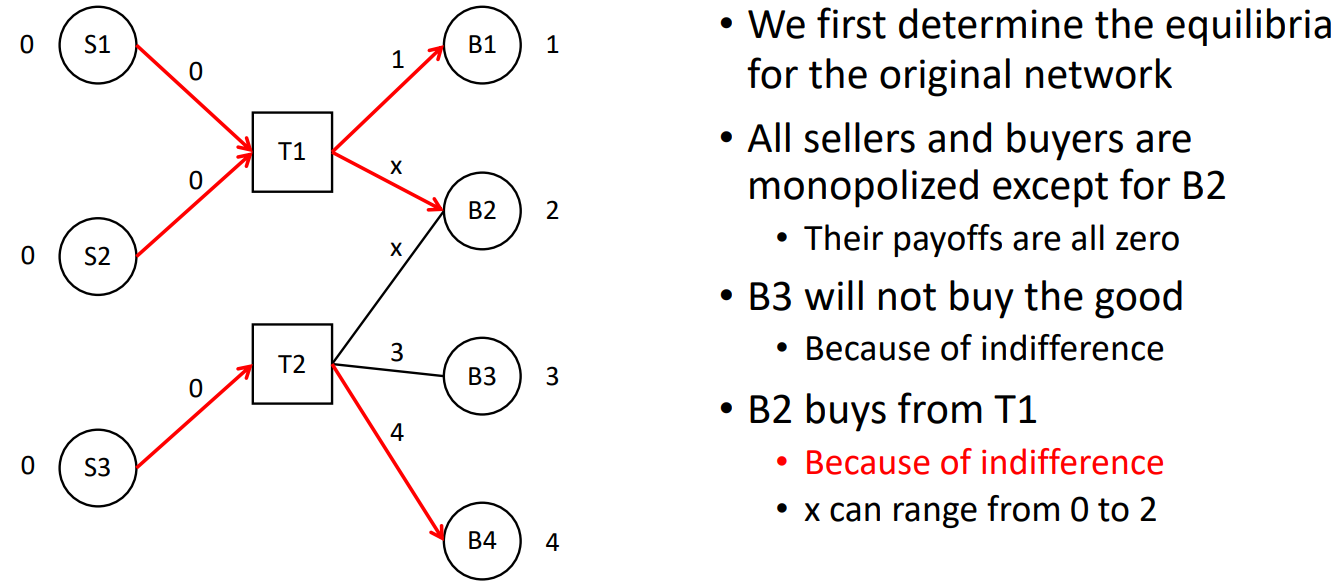
\includegraphics[width=0.6\textwidth]{ripple_1}
\end{figure}

\begin{figure}[H]
    \centering
    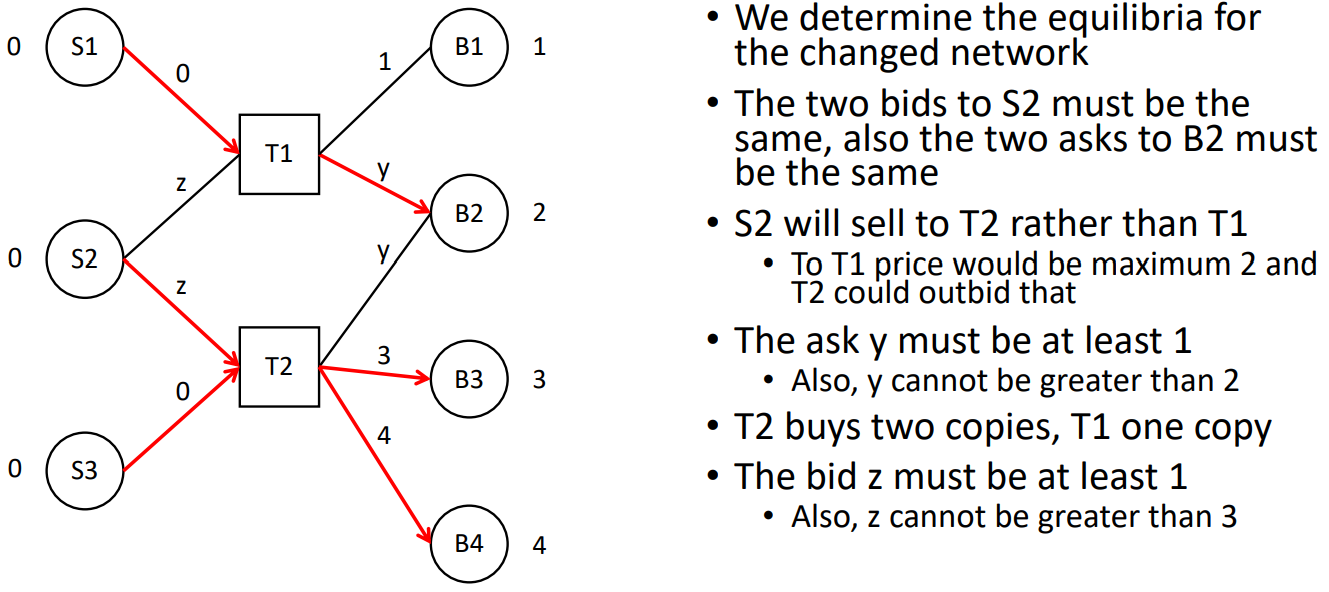
\includegraphics[width=0.6\textwidth]{ripple_2}
\end{figure}

\subsection{Social welfare in trading networks}

\begin{itemize}
\item The \textcolor{orange}{social welfare} is simply the \textcolor{orange}{sum of $(v_j - v_i)$} over all moved goods.
\item There \textcolor{orange}{exist values for the variable that maximize social welfare} and picks an equilibrium.
\item In every trading network, \textcolor{orange}{there is always at least one equilibrium}.
\item \textcolor{orange}{Social welfare increases as connectivity increases.}
\end{itemize}

\subsection{Summary}

\begin{figure}[H]
    \centering
    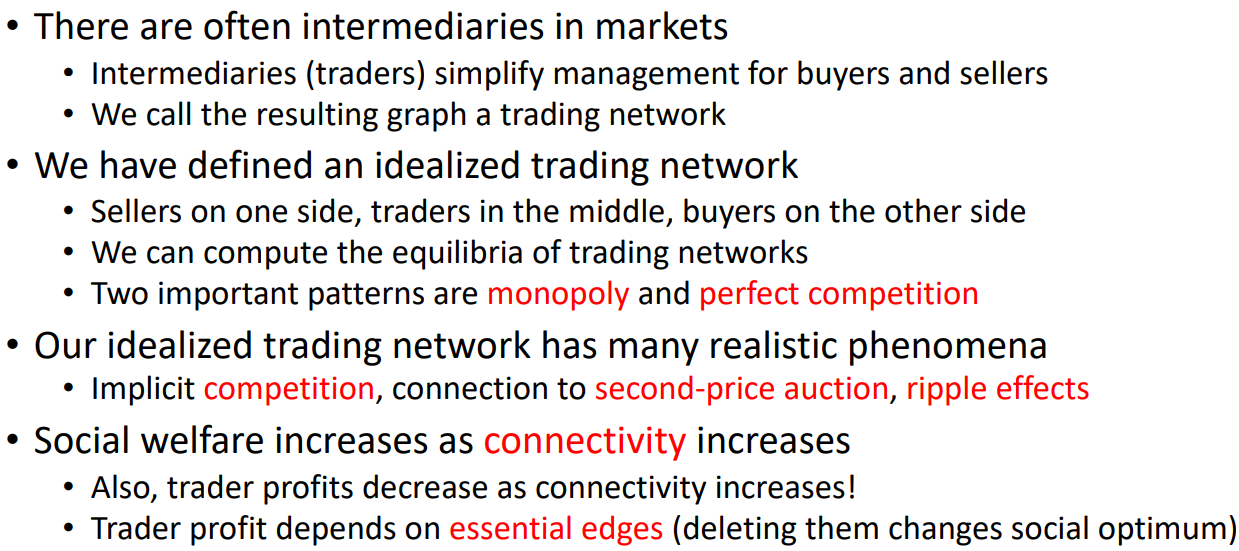
\includegraphics[width=0.7\textwidth]{trading_networks_sum}
\end{figure}

\section{Bargaining and power in networks}

\subsection{Power in paths}

\begin{figure}[H]
    \centering
    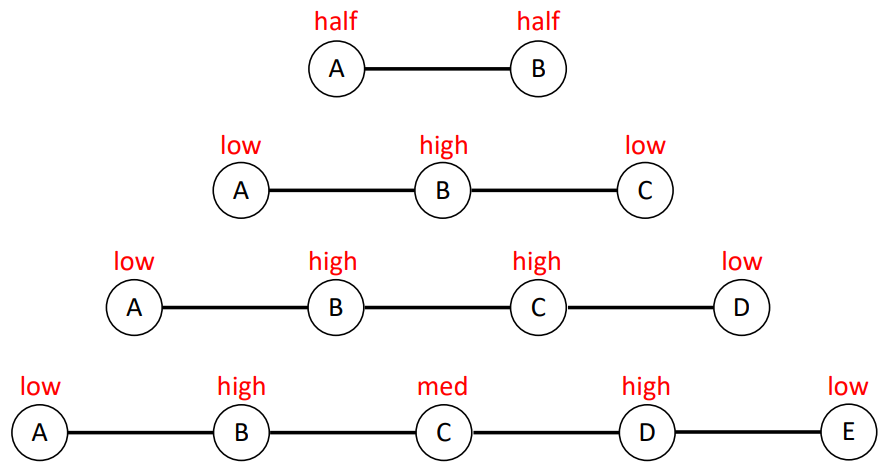
\includegraphics[width=0.7\textwidth]{power_path}
\end{figure}

\subsection{A mathematical framework for negotiation}

\subsubsection{Nash bargaining solution}

\begin{figure}[H]
    \centering
    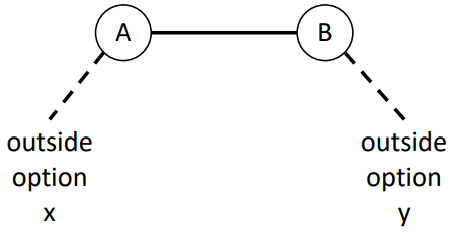
\includegraphics[width=0.3\textwidth]{nash_bargaining}
\end{figure}

\begin{itemize}
\item A gets $x + (s/2)$ and B gets $y + (s/2)$ where $s = 1 - x - y$.
\item Nash bargaining solution :
	\begin{enumerate}
	\item A gets $(x + 1 - y)/2$
	\item B gets $(y + 1 - x)/2$
	\end{enumerate}
\end{itemize}

\subsubsection{Ultimatum game}

\begin{enumerate}
\item A is given a dollar and is told to propose a division with B, that is, A proposes how much to keep from himself and how much to give to B.
\item B is given the option to approve or reject the division.
\item if B approves, both get the proposed amount. If B rejects, both get zero.
\end{enumerate}

\paragraph{Game theory}

Game theory says that B should accept if the amount $> 0$.

\paragraph{Human way of playing}

\begin{itemize}
\item If the amount offered is to unbalanced, B will feel cheated and will refuse A's offer.
\item We say there is an \textcolor{orange}{Emotional payoff}.
\end{itemize}

\subsubsection{Stable outcomes}

\begin{itemize}
\item An outcome of a network is stable if and only if it contains no instabilities.
\item Stability is too weak in networks with small power difference
\end{itemize}

\paragraph{Outcome of a network exchange on a graph}

\begin{enumerate}
\item A matching on the set of nodes. This corresponds to the one-exchange rule, and some nodes may be left out.
\item A number associated with each node, its value, indicating how much the node gets from the exchange. If two nodes are matched, the sum of values should be $1$. If a node is not in a matching, its value should be $0$.
\end{enumerate}

\paragraph{Instability}

Given an outcome consisting of a matching and set of values, an instability in this outcome is an edge not in the matching, joining two nodes $X$ and $Y$, such that $(X$’s value$) + (Y$’s value$) < 1$.

\subsubsection{Theory of balanced outcomes}

\begin{formal}
An outcome (consisting of a matching plus node values) is balanced, if for each edge in the matching, the money split represents the Nash bargaining solution for the two nodes involved, given the best outside options for each node provided by the values in the rest of the network.
\end{formal}

\begin{figure}[H]
    \centering
    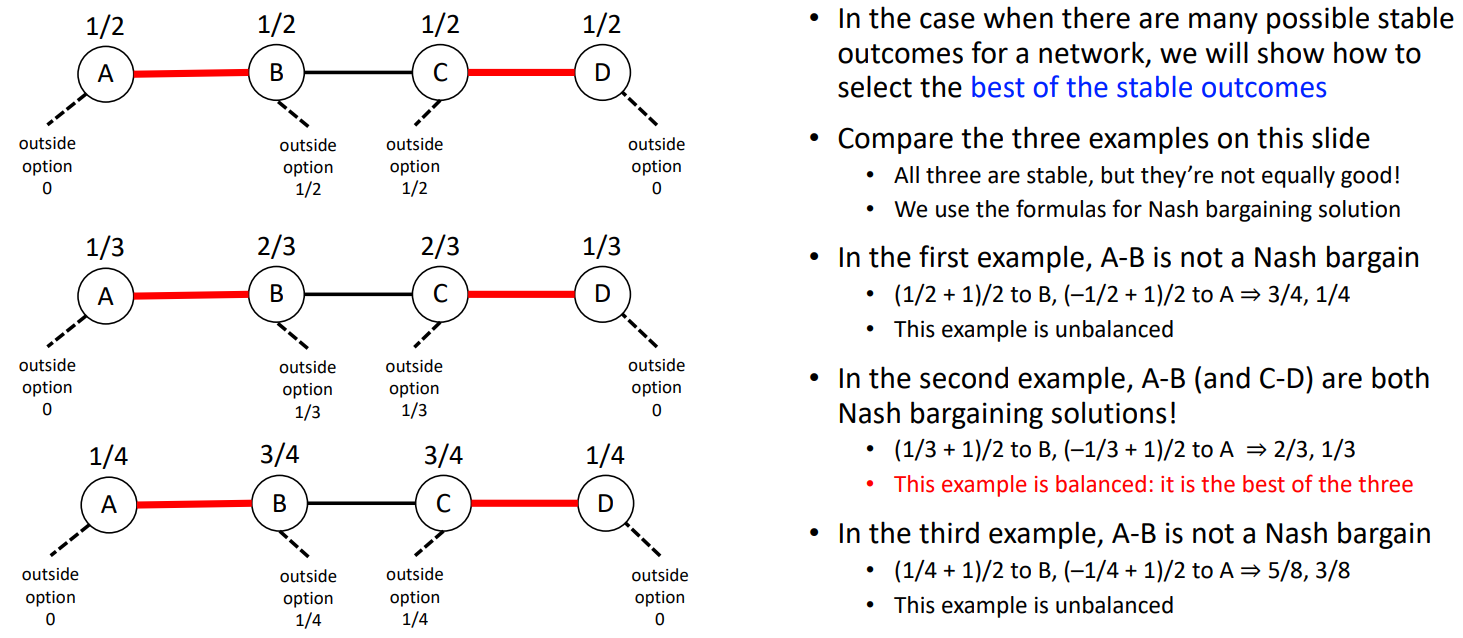
\includegraphics[width=0.7\textwidth]{balanced_outcomes}
\end{figure}

Outcome is balanced when all agreements are Nash bargaining solutions; balanced outcomes exist whenever stable outcomes exist.

\subsection{Summary}

\begin{figure}[H]
    \centering
    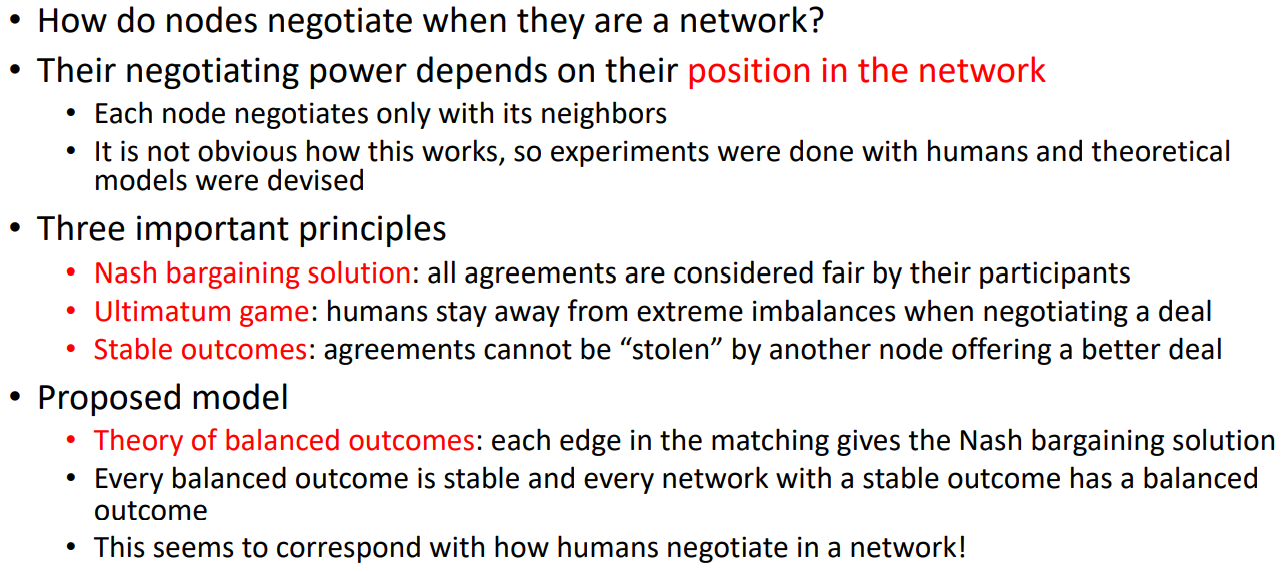
\includegraphics[width=0.7\textwidth]{negotiation_network}
\end{figure}

\chapter{World Wide Web}

\section{Structure of the web}

\subsection{Hypertext}

Each node is a page that contains links to other pages.

\subsection{Network distribution}

Pages are geographically distributed as internet nodes.

\subsection{Bow-tie structure}

\begin{figure}[H]
    \centering
    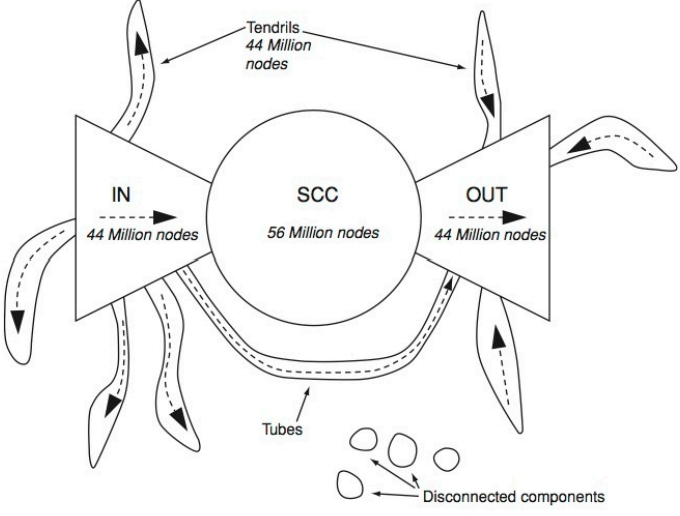
\includegraphics[width=0.5\textwidth]{bow_tie_web}
\end{figure}

\textcolor{orange}{SCC}: Strongly connected component

\section{Web 2.0}

\subsection{Increased abstraction level}

\begin{enumerate}
\item Collaborative creation and maintenance of shared content, instead of individuals creating pages (Wikipedia).
\item Creation of services that manage data, instead of sets of pages (Gmail).
\item Connections between people instead of between pages (Facebook).
\end{enumerate}

\subsection{Social phenomena}

\subsubsection{Software that gets better the more people use it}

Online services are more useful and more appealing as more people use them. A marketplace is more useful as more people put objects for sale and more buy objects. Recommendation systems and trust systems are more useful as more people use them.

\subsubsection{The wisdom of crowds}

Collaborative authorship on Wikipedia, group evaluation of news content on Digg, breaking news on Twitter. This process can also fail, because of herding and instability.

\subsubsection{The "Long Tail"}

Combining a small amount of very popular content with a huge amount of less popular content with “niche appeal”. The less popular content is often bigger than the popular content.

\section{Link analysis and Web search}

\subsection{The problem of search}

\begin{itemize}
\item \textcolor{orange}{Inexpressiveness} : subtle ideas cannot be expressed using keyword combinations.
\item \textcolor{orange}{Synonymy} : multiple words for the same concept, "scallions" vs "green onions".
\item \textcolor{orange}{Polysemy} : the same word has multiple meanings, "jaguar" gives cars instead of animals.
\item \textcolor{orange}{Abundance problem} : too much relevant information.
\end{itemize}

\subsection{Hubs and authorities}

\begin{itemize}
\item \textcolor{orange}{Authority} : page we are looking for, a high-quality answer to the query.
\item \textcolor{orange}{Hub} : page that has a high-quality list to the pages we are looking for.
\end{itemize}

\subsubsection{Algorithm to compute scores}

\begin{itemize}
\item Start with all hub and authority scores equal to 1.
\item Repeat $k$ times :
	\begin{itemize}
	\item For each page $p$, update auth($p$) to be the sum of all hubs pointing to it.
	\item For each page $p$, update hub($p$) to be the sum of all authority pages it points to.
	\item Normalize the authority scores by dividing by sum o all authorities (and also for hubs).
	\end{itemize}
\end{itemize}

\subsubsection{Limiting values}

\begin{itemize}
\item Limiting values re \textcolor{orange}{independent of the initial values} of hub ad authority scores.
\item The \textcolor{orange}{normalized values converge to limits}.
\end{itemize}

\subsection{PageRank}

\begin{itemize}
\item Uses only \textcolor{orange}{one value per page} and it is its \textcolor{orange}{importance}.
\item Intuitively the \textcolor{orange}{PageRank} value is a kind of "fluid" that circulates through the network, where nodes are containers and links are pages.
	\begin{itemize}
	\item[$\rightarrow$] The amount of fluid is \textcolor{orange}{constant}, so \textcolor{orange}{normalization is automatic}.
	\end{itemize}
\end{itemize}

\subsubsection{Basic algorithm}

\paragraph{Initialization}

We assume that the network has n nodes.
\begin{itemize}
\item[$\rightarrow$] $\forall p : pr(p) := \frac{1}{n}$
\end{itemize}

\paragraph{Iteration}

\begin{enumerate}
\item Compute the amount of fluid on outgoing links of all pages $p$.
	\begin{itemize}
	\item[$\rightarrow$] $\forall p : pr_{\text{link}}(p, p') := \frac{pr(p)}{m}$ (page $p$ has $m$ outgoing links, each to $p'$)
	\end{itemize}
\item Sum all fluid for incoming links of page $p$.
	\begin{itemize}
	\item[$\rightarrow$] $\forall p : pr(p) := \sum_{p'} \text{incoming links } pr_{\text{link}}(p, p')$
	\end{itemize}
\end{enumerate}

\paragraph{Problem with the basic definition}

Some nodes can collect all the PageRank values.

\paragraph{Fixing the problem}

\begin{enumerate}
\item Apply the basic update rule.
\item Do the following scaling : $\forall p : pr(p) := s * pr(p) + \frac{1 - s}{n}$
	\begin{itemize}
	\item This uses scaling factor $s$ strictly between $0$ and $1$ (often $0.8$ or $0.9$). The PageRank fraction $(1-s)$ “evaporates” from each node and “rains” uniformly on all nodes.
	\item This completes the cycle between all nodes.
	\end{itemize}
\end{enumerate}

\subsubsection{Random walk definition}

\begin{itemize}
\item Consider a person randomly browsing the Web :
	\begin{itemize}
	\item They start by picking a page at random (each page equal probability).
	\item They follow links for $k$ steps and in each step they follow a random link.
		\begin{itemize}
		\item[$\rightarrow$] This is called a random walk on the network.
		\end{itemize}
	\item We can prove that the probability of being on a page $X$ after $k$ steps is precisely the PageRank of $X$ after $k$ iterations of the basic update rule.
	\end{itemize}
\item The scaled update rule is formulated as follow :
	\begin{itemize}
	\item At each step, the walker follows a random link with probability $s$, and "jumps" to a random page with probability $(1-s)$.
	\item The walker mostly follows the link and sometimes jumps.
	\end{itemize}
\end{itemize}

\section{Summary}

\begin{figure}[H]
    \centering
    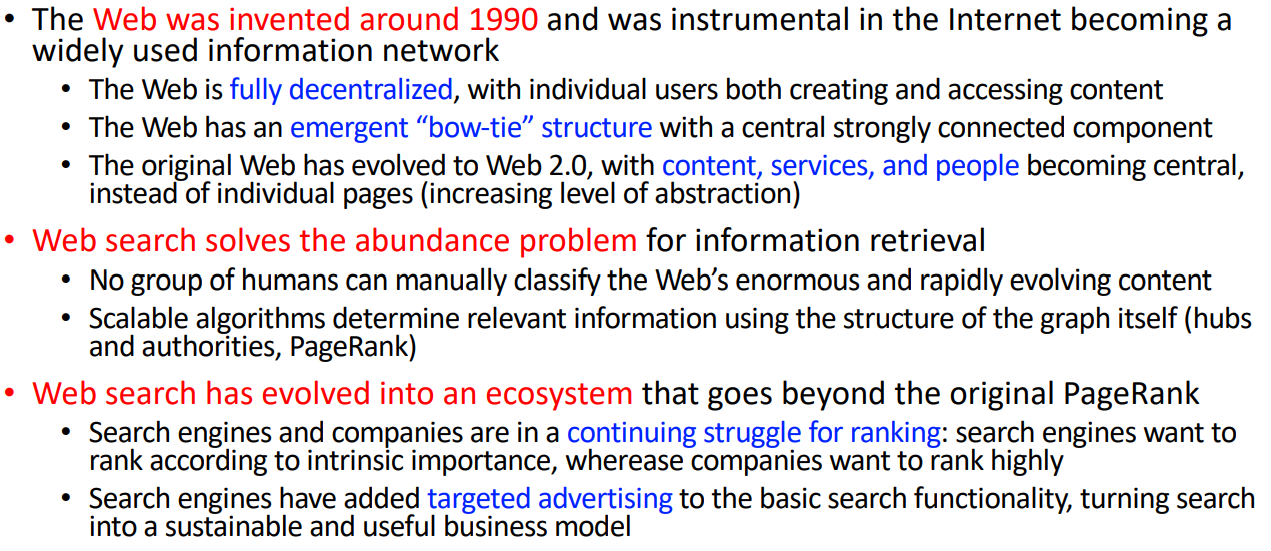
\includegraphics[width=0.8\textwidth]{web_sum}
\end{figure}
